\section{Implementazione in PostgreSQL e Definizione
delle Query}

\subsection{Definizione delle Query}

1. \textbf{QUERY 1} Media del costo dei pacchi di un corriere di un certo grado che sono passati per una filiale di un certo tipo
  \begin{figure}[H]
\centering
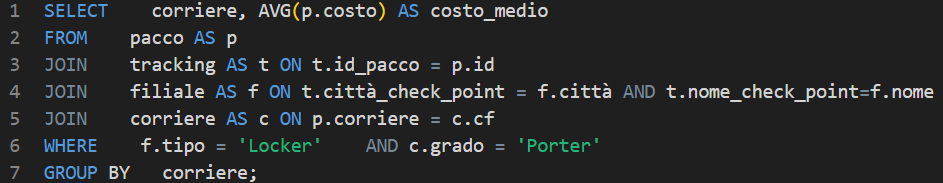
\includegraphics[width=0.8 \textwidth]{Resources/QUERY1.png}
\label{ML}
\end{figure}
2. \textbf{QUERY 2} Numero pacchi per bundle con garanzia 3 anni
\begin{figure}[H]
\centering
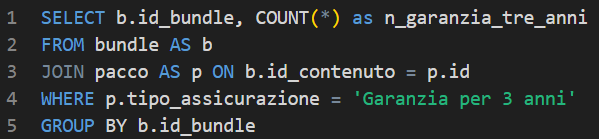
\includegraphics[width=0.8 \textwidth]{Resources/QUERY2.png}
\label{ML}
\end{figure}
3. \textbf{QUERY 3} Corrieri che hanno un tempo di consegna medio dei loro pacchi superiore al tempo medio di consegna di un pacco:
\begin{figure}[H]
\centering
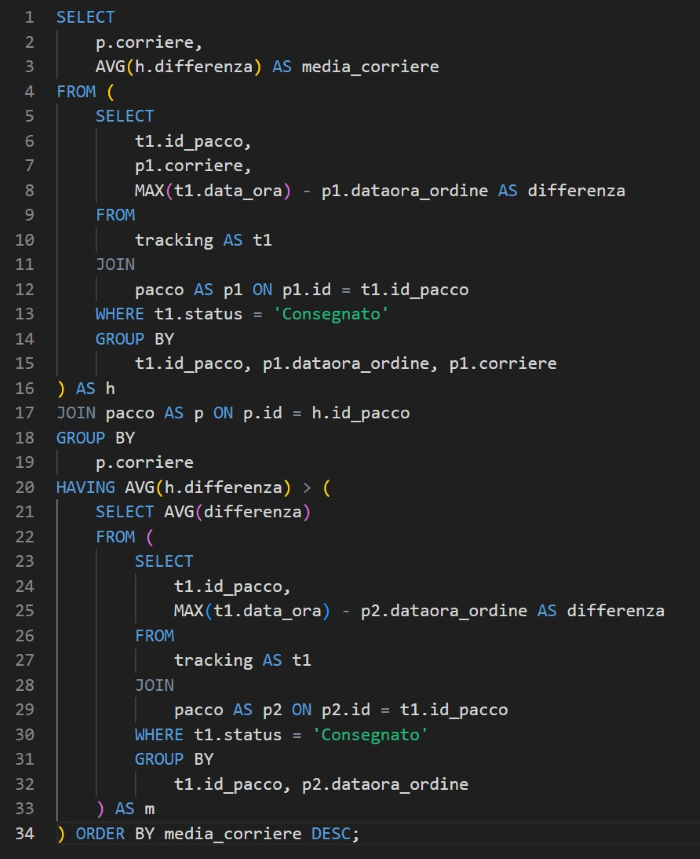
\includegraphics[width=0.6 \textwidth]{Resources/QUERY3.png}
\label{ML}
\end{figure}
4. \textbf{QUERY 4} Corrieri con bundle con pacchi con garanzia a 3 anni e costo maggiore di 300
\begin{figure}[H]
\centering
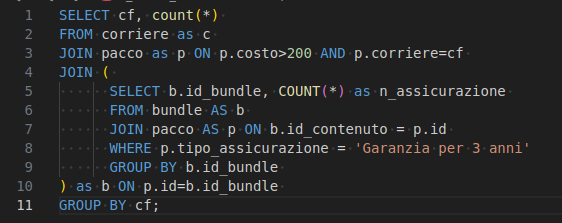
\includegraphics[width=0.8 \textwidth]{Resources/QUERY4.png}
\label{ML}
\end{figure} 
5. \textbf{QUERY 5} Ultimo aggiornamento del tracking di un pacco
\begin{figure}[H]
\centering
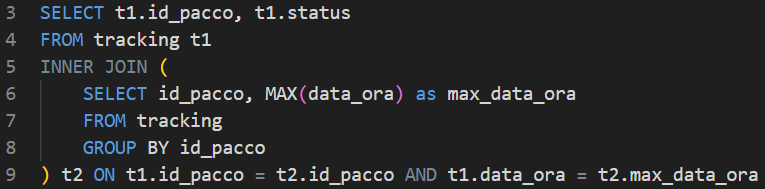
\includegraphics[width=0.8 \textwidth]{Resources/QUERY5.png}
\label{ML}
\end{figure}

\subsection{Creazione degli Indici} 

Supponendo di voler ottimizzare la query num 5, si deve considerare:

\begin{itemize}
  \item Condizione del JOIN: \texttt{t.id\_pacco = p.id}
  \item Condizione del JOIN: \texttt{t.città\_check\_point = f.città AND t.nome\_check\_point = f.nome}
  \item Condizione del JOIN: \texttt{p.corriere = c.cf}
  \item Condizione del WHERE: \texttt{ f.tipo = 'Locker'AND c.grado = 'Porter'}
  \item GROUP BY sulle colonne: \texttt{corriere}
\end{itemize}


\noindent Per il punto 1 è opportuno creare due indici hash su entrambe le colonne del join:
\begin{figure}[H]
\centering
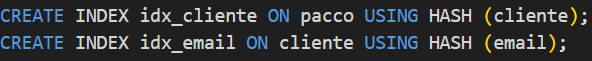
\includegraphics[width=0.8 \textwidth]{Resources/INDEX1.png}
\label{ML}
\end{figure}

\noindent Per il punto 2 è opportuno creare quattro indici hash per tutte le condizioni del join:
\begin{figure}[H]
\centering
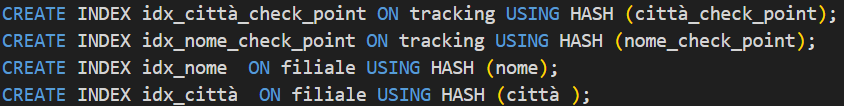
\includegraphics[width=0.8 \textwidth]{Resources/INDEX2.png}
\label{ML}
\end{figure}

\noindent Per il punto 3 è opportuno creare due indici hash su entrambe le colonne del join:

\begin{figure}[H]
\centering
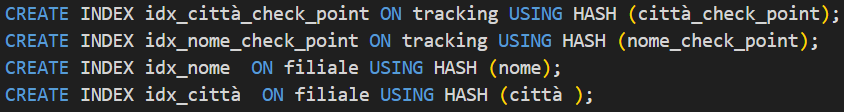
\includegraphics[width=0.8 \textwidth]{Resources/INDEX3.png}
\label{ML}
\end{figure}

\noindent Per il punto 4 è opportuno creare due indici per i due attributi rispetto a cui il WHERE valuta la sua condizione:

\begin{figure}[H]
\centering
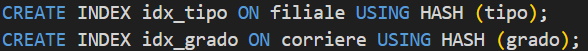
\includegraphics[width=1 \textwidth]{Resources/INDEX4.png}
\label{ML}
\end{figure}

\noindent Il punto 5 è un GROUP BY e potrebbe quindi essere ottimizzato tramite il seguente indice B+Tree:
 
\begin{figure}[H]
\centering
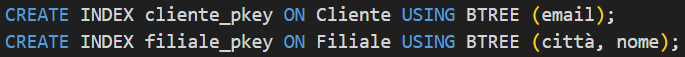
\includegraphics[width=1 \textwidth]{Resources/INDEX5.png}
\label{ML}
\end{figure}  

\noindent Visto che non si tratta di un attributo che è chiave primaria di una entità POSTGRE non ha già creato l'indice corrispondente. 